\documentclass[french, a4paper, 12pt, titlepage]{article}
%% Peut remplacer "article" par "scrartcl" %%

\usepackage[french]{babel}
\usepackage{a4wide}
%\usepackage[top=2cm, bottom=2cm, left=2cm, right=2cm]{geometry}
\raggedbottom % prevents vertical white space on pages that cannot be filled properly

\usepackage{hyperref}
\hypersetup{
	colorlinks=true,       	% false: boxed links; true: colored links
	linkcolor=black,          	% color of internal links
	urlcolor=blue,           	% color of external links
	citecolor=grey
}

\usepackage[T1]{fontenc}
%\usepackage{fourier}
%\usepackage{utopia}
%\usepackage{palatino}

\usepackage{lmodern}
%% ajouter fonte petite capitale grasse à lmodern avec celle de computer modern %%
\rmfamily
\DeclareFontShape{T1}{lmr}{b}{sc}{<->ssub*cmr/bx/sc}{}
\DeclareFontShape{T1}{lmr}{bx}{sc}{<->ssub*cmr/bx/sc}{}
%% /ajout %%
\usepackage{wrapfig}

%\usepackage[a4paper]{geometry} % marges plus petites que a4paper standard
\usepackage{listings} % insérer code source
\lstloadlanguages{sh,bash,awk,make}
%\usepackage{algorithm} % algorithmique
%\usepackage{algorithmic}
\usepackage{url}
\usepackage[usenames, dvipsnames]{color} % couleurs (nombre de base étendu)
\usepackage{graphicx} % insérer images
\usepackage[utf8]{inputenc}
\usepackage{amsmath}
\usepackage{amsfonts}
\usepackage{amssymb}
\usepackage{amsthm}
\usepackage{multicol}
\usepackage{dirtree}
\definecolor{grey}{rgb}{0.96,0.96,0.96}
\definecolor{grey2}{rgb}{0.3,0.3,0.3}

%% Define listings params %%
\lstset{
%	numbers=left,
	language=bash,
	tabsize=4,
	frame=single, % cadre autour du code
	breaklines=true, % autorise couper ligne trop longue
	basicstyle=\small\ttfamily,
	numberstyle=\scriptsize\ttfamily,
	backgroundcolor=\color{grey},
	showstringspaces=false,
	keywordstyle=\color{OliveGreen},
	stringstyle=\color{BrickRed},
	commentstyle=\color{grey2}\it,
	stepnumber=1 % numérote toute les x lignes
}
% listing utf8 fr %
\lstset{%
	inputencoding=utf8,
	extendedchars=true,
	literate=
		{é}{{\'{e}}}1
		{è}{{\`{e}}}1
		{ê}{{\^{e}}}1
		{ë}{{\¨{e}}}1
		{û}{{\^{u}}}1
		{ù}{{\`{u}}}1
		{â}{{\^{a}}}1
		{à}{{\`{a}}}1
		{î}{{\^{i}}}1
		{ç}{{\c{c}}}1
		{Ç}{{\c{C}}}1
		{É}{{\'{E}}}1
		{Ê}{{\^{E}}}1
		{À}{{\`{A}}}1
		{Â}{{\^{A}}}1
		{Î}{{\^{I}}}1
}
%% /Define listings params %%

%% Francisation des algorithmes
%\renewcommand{\algorithmicrequire} {\textbf{\textsc{Entrées:}}}
%\renewcommand{\algorithmicensure}  {\textbf{\textsc{Sorties:}}}
%\renewcommand{\algorithmicwhile}   {\textbf{tant que}}
%\renewcommand{\algorithmicdo}      {\textbf{faire}}
%\renewcommand{\algorithmicendwhile}{\textbf{fin tant que}}
%\renewcommand{\algorithmicend}     {\textbf{fin}}
%\renewcommand{\algorithmicif}      {\textbf{si}}
%\renewcommand{\algorithmicendif}   {\textbf{fin si}}
%\renewcommand{\algorithmicelse}    {\textbf{sinon}}
%\renewcommand{\algorithmicthen}    {\textbf{alors}}
%\renewcommand{\algorithmicfor}     {\textbf{pour}}
%\renewcommand{\algorithmicforall}  {\textbf{pour tout}}
%\renewcommand{\algorithmicdo}      {\textbf{faire}}
%\renewcommand{\algorithmicendfor}  {\textbf{fin pour}}
%\renewcommand{\algorithmicloop}    {\textbf{boucler}}
%\renewcommand{\algorithmicendloop} {\textbf{fin boucle}}
%\renewcommand{\algorithmicrepeat}  {\textbf{répéter}}
%\renewcommand{\algorithmicuntil}   {\textbf{jusqu'à}}
%\renewcommand{\algorithmiccomment} {\STATE //}
%\newcommand{\BEGIN}{\STATE \fbox{Début}}
%\newcommand{\END}{\STATE \fbox{Fin}}
%\floatname{algorithm}{Algorithme}
%% /francisation des algorithmes

\renewcommand{\qedsymbol}{}

\newcommand{\petit}[1]{
	\medskip \noindent
	\begin{small}
	#1)
	\end{small}
}

\begin{document}

\title{Introduction aux commandes shell (Linux) basique}
\author{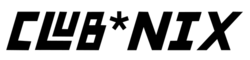
\includegraphics[scale=0.7]{clubnix}}
\date{\url{https://github.com/ClubNix/man-terminal}}

\maketitle
%% Laisse page blanche pour verso page de garde %%

\vfill
\pagebreak
\newpage
\thispagestyle{empty}
~

%\tableofcontents

\strut\thispagestyle{empty}
\vfill
\pagebreak
\tableofcontents
\strut\thispagestyle{empty}

%\setcounter{page}{0}
\vfill
\pagebreak
\newpage
\thispagestyle{empty}
~
\pagebreak

\setcounter{page}{1}

\part{Presentation d'un environnement GNU/Linux}

\paragraph{}
Le projet \textit{GNU/Linux} commence en 1983 lorsque Richard Stallman propose
de développer un ensemble de logiciels libres, s'appelant le projet GNU, mais
ce n'est qu'en 1992 après avoir fini la plupart des outils essentiels que Linus
Torvalds propose un kernel (le cœur d'un système d'exploitation),
\textit{Linux}, et ceci permet donc de lancer un système exempt de tout
logiciel propriétaire.

\paragraph{}
A l'heure actuelle, GNU/Linux est essentiellement utilisé en tant que serveur
dans des sociétés comme Google, Amazon, Facebook, Twitter et bien d'autre.
GNU/Linux est aussi la technologie utilisée dans les téléphones Android, dans
beaucoup de machines comme les distributeurs de billets ou les télévisions, ou
de manière générale un grand nombre de systèmes embarqués, mais aussi par des
personnes qui l'utilisent comme ordinateur pour la vie courante.

\paragraph{}
Pour la petite histoire, le logo de Linux n'est pas un pingouin mais un
\textbf{manchot}, plus exactement un manchot pygmée, qui porte le nom de
\textbf{Tux}. Linus est en effet revenu avec cette idée de mascotte après
s'être fait mordre lors d'un voyage en Australie par cette même espèce de
manchot et coupa court à la discussion qui se portait sur un requin.

\part{Qu'est-ce que le terminal?}

\paragraph{} Pour comprendre ce qu'est le terminal, il faut d'abord savoir
qu'il y a deux catégories de programmes: les programmes graphiques et les
programmes en mode texte. Un inconvénient des programmes en mode texte: ils ont
besoin d'un "support" où le texte va être affiché. On appelle ce support un
terminal.

\paragraph{} Pour lancer la bête, vous pouvez tester les différentes solutions
suivantes:
\begin{itemize}
	\item Menu $\rightarrow$ barre de recherche $\rightarrow$ "terminal" (ou
		"konsole" ou "gnome-terminal" ou "xfterm4" ou "xfce4-terminal")
	\item application $\rightarrow$ accessoires $\rightarrow$ terminal
	\item <super> $\rightarrow$ taper "terminal"
	\item Alt + f2 $\rightarrow$ taper "gnome-terminal"
	\item Ctrl+Alt+T
	\item sinon le logo à rechercher ressemble à ça:
		
\includegraphics[scale=0.7]{Images/termIcon}
\end{itemize}

\paragraph{} Le terminal peut vous faire peur et picoter les yeux au premier
abord, mais n'ayez crainte. Commençons par ce picotement des yeux,
en faisant un clic droit et en allant dans profils, préférences du profil vous
pourrez changer la couleur pour quelque chose de moins agressif pour vos yeux,
"blanc sur noir" ou "vert sur noir" (pour les plus geeks d'entre vous)
plusieurs choses peuvent être configurées, je vous laisse les découvrir.

\paragraph{} Ce que vous pouvez voir à partir de là est une ligne ressemblant à
ceci :
\begin{lstlisting}
user@pc ~ $
\end{lstlisting}

%PS1="\[\033[01;32m\]club@nix\[\033[01;34m\] \w \$\[\033[00m\] "

\begin{center}
	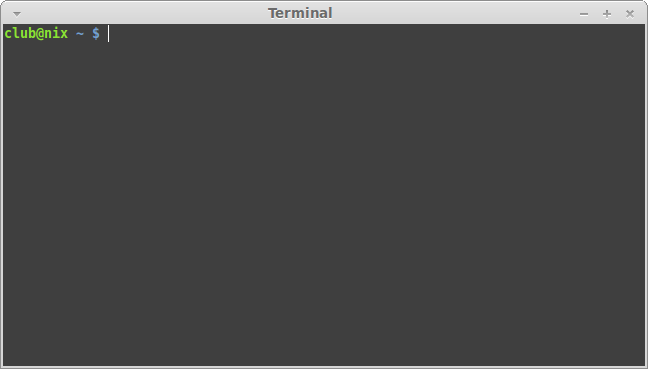
\includegraphics[scale=0.42]{Images/terminal}
\end{center}

\paragraph{} Le programme qui affiche du texte dans le terminal est ce qu'on
appelle un \emph{Shell}, et il va vous permettre d'entrer des commandes
GNU/Linux. Vous avez aussi l'affichage d'un certain nombre d'informations
utiles:

\begin{enumerate}
	\item[user@pc] correspond à votre login (nom d'utilisateur, ici
		<<~user~>>) suivi du nom de la machine (ici <<~pc~>>) sur laquelle
		vous vous trouvez, le tout est séparé par le caractère <<~@~>>.
	\item[$\sim$] est le dossier courant suivit du caractère "\$"
		(le dossier $\sim$ est un raccourci vers votre dossier personnel
		\emph{/home/user/}).
	\item[\$] Le dollar signifie juste que vous êtes un utilisateur normal (à
		l'opposition du \emph{\#} qui signifie que vous êtes
		super-utilisateur).
\end{enumerate}

\paragraph{} Il existe toutes sortes de Shell (bash, tcsh, sh, ksh, zsh\dots)
qui ont chacun des fonctionnalités différentes, mais tous permettent d'exécuter
des commandes ou des programmes. Dans le monde réel, \emph{bash} est
l'interpréteur le plus courant, cependant pour une raison obscure, vous
commencerez par défaut votre aventure à l'ESIEE avec \emph{tcsh}.

\paragraph{} Comme \emph{tcsh} est très peu convivial, nous supposerons par la
suite que vous utilisez bash (vous pouvez lancer \emph{bash} à l'intérieur du
terminal en tapant la commande \texttt{bash}).

\paragraph{} En résumé, le Shell correspond au programme qui va interpréter et
exécuter les commandes tapées à l'intérieur de votre terminal. Il est composé
de texte, qui affiche des informations utiles, un d'un champ de texte qui vous
permet d'entrer des commandes en tapant sur le clavier. C'est donc est
l'interface minimale entre l'utilisateur et le système d'exploitation.

\paragraph{} Le Shell est exécuté à l'intérieur d'un terminal qui est une
application graphique qui permet de faire l'intermédiaire entre les programmes
en mode texte et l'utilisateur.

\part{Notation}

\begin{enumerate}
	\item[\^{}] correspond à la touche <<~\emph{Ctrl}~>>, \^{}C, signfie donc
		qu'il faut appuyer en même temps sur la touche "Ctrl" et C (deux
		touches sont enfoncées).
	\item [<super>] correspond à la touche "super" honteusement surmontée par
		un logo windows sur la plupart des claviers.
	\item [M-] correspond à la touche "Meta", le "alt" à côté de la touche
		espace.
\end{enumerate}

\part{Chemins absolus et chemins relatifs}

\paragraph{} Un chemin, ou chemin d'accès (\emph{path} en anglais) représente
tout simplement la position d'un fichier ou d'un dossier dans le système. Sous
GNU/Linux, les chemins sont séparés par des barres obliques orientés vers la
droite: ``\texttt{/}''.  Cela explique le fait que ce caractère soit interdit
dans les noms de fichiers et dossiers sous GNU/Linux.

\paragraph{Exemples:}

\begin{itemize}
	\item \texttt{/home/nom-d-utilisateur/Documents/Bla.pdf}
	\item \texttt{Musique/thing.mp3}
	\item \texttt{\~{}/Images/wallpaper.png}
	\item \texttt{../man-terminal.pdf}
\end{itemize}

\section{Chemins absolus}

\paragraph{} Les chemins absolus sont des chemins qui prennent comme point de
départ la racine du système (\emph{root} en anglais) dont tout les fichiers et
dossiers sont des descendants. Un chemin relatif commencera toujours par un
\emph{slash} (``\texttt{/}'').

\paragraph{} Ainsi, \texttt{/home/nom-d-utilisateur/Documents/Bla.pdf}
représente le fichier \texttt{Bla.pdf} qui est situé dans le dossier
\texttt{Documents}, lui-même étant dans le dossier \texttt{nom-d-utilisateur},
lui-même contenu dans le dossier \texttt{home} qui est un descendant direct du
dossier racine. Cela donne donc (en omettant les autres dossiers et fichiers):
\\
\dirtree{%
	.1 / (root).
		.2 home.
			.3 nom-d-utilisateur.
				.4 Documents.
					.5 Bla.pdf.
}

\section{Chemins relatifs}

\paragraph{} Les chemins relatifs, à la différence des chemins absolus,
prennent en compte le dossiers dans lequel on est. Ainsi, un chemin relatif ne
mènera pas au même fichier selon où l'on est. Ces types de chemins sont très
utiles pour les fainéants qui ne veulent pas tout re-taper depuis le dossier
racine. Les chemins relatifs ne commencent pas par un \emph{slash}.

\paragraph{} Par exemple, \texttt{Musique/thing.mp3} représente le fichier
\texttt{thing.mp3} qui est dans le dossier \texttt{Musique} lui même qui est
dans le dossier actuel. En supposant que le dossier actuel soit le dossier
personnel (\texttt{/home/nom-d-utilisateur}), cela nous donne:
\\
\dirtree{%
	.1 / (root).
		.2 home.
			.3 nom-d-utilisateur (dossier actuel).
				.4 Musique.
					.5 thing.mp3.
}

\section{Chemins spéciaux}

\paragraph{} Parmis les chemins sous GNU/Linux, il y a quelques chemins
spéciaux:

\begin{itemize}
	\item ``\texttt{\~}'' correspond au dossier personnel
		(\texttt{/home/nom-d-utilisateur}), ainsi\\
		\texttt{\~/Musique}\\
		correspond à\\
		\texttt{/home/nom-d-utilisateur/Musique}
	\item ``\texttt{.}'' correspond au dossier actuel, donc\\
		\texttt{Documents/./texte.txt}\\
		correspond à\\
		\texttt{Documents/texte.txt}
	\item ``\texttt{..}'' correspond au dossier parent, donc\\
		\texttt{/home/nom-d-utilisateur/Documents/../Téléchargements/cat.gif}\\
		est équivalent à\\
		\texttt{/home/nom-d-utilisateur/Téléchargements/cat.gif}
\end{itemize}

\section{Caractères spéciaux}

\paragraph{} Sous GNU/Linux, le seul caractère présent sur le clavier non
autorisé dans les noms de fichiers et dossiers est le \emph{slash}. Cependant
il existe d'autres caractères spéciaux pour le shell qui devront être
\emph{échappés}, ce qui veut dire qu'il devront être précédés d'un
\emph{antislash} (``\texttt{\textbackslash}''). Les plus utilisés sont:

\begin{itemize}
	\item \textvisiblespace~(l'espace)
	\item \texttt{"}
	\item \texttt{'}
	\item \texttt{!}
	\item \texttt{\#}
	\item \texttt{\$}
	\item \texttt{(}, \texttt{)}, \texttt{[}, \texttt{]}, \texttt{\{}, \texttt{\}}
\end{itemize}

\paragraph{} Donc si un fichier s'appelle \texttt{Un nom trè\$ embêtant (mais
peu probable)}, on devra écrire dans le \emph{prompt}:
\texttt{Un\textbackslash{\textvisiblespace}nom\textbackslash{\textvisiblespace}trè\textbackslash\$\textbackslash\textvisiblespace
embêtant\textbackslash{\textvisiblespace}\textbackslash(mais\textbackslash{\textvisiblespace}peu\textbackslash
probable\textbackslash)}.

\paragraph{} Un moyen d'éviter ceci est de mettre guillemets (simples ou
doubles) autour. Prenez garde tout de même car le symbole du dollar doit
quand-même être échappé si l'on met des guillemets doubles. Pour notre exemple,
cela donne:
\\
\begin{itemize}
	\item \texttt{"Un nom trè\textbackslash\$ embêtant (mais peu probable)"}\\
	ou
	\item \texttt{'Un nom trè\$ embêtant (mais peu probable)'}
\end{itemize}

\part{Commandes Basiques (débutant)}

\section{Raccourcis utiles}

\begin{description}
	\item[Entrée]: la plus importante, lance votre commande
	\item[Flêche haut]: naviguer dans l'historique des commandes. Vous pourrez
		ainsi gagner du temps et éviter de retaper toujours la même chose.
	\item[Tab]: touche de complétion. Vous permet de taper les quelques
		premières lettres de votre commande, puis les compléter en appuyant sur
		la touche de tabulation. Si rien ne s'affiche la première fois que vous
		appuyez sur la touche, c'est qu'il existe plusieurs possibilités de
		complétion. Une seconde pression vous permettra d'afficher toutes les
		complétions possibles.
	% TODO: move that to job control section
	% \item[Ctrl + Z]: pause la commande en cours.
	\item[Ctrl + C]: arrête la commande en cours et recommence avec une
		nouvelle ligne. Très utile si vous voulez annuler l'exécution d'un
		programme qui boucle de manière infinie, ou si vous vous rendez compte
		que vous êtes en train d'écrire n'importe quoi.
	\item[Ctrl+L]: nettoie l'écran.
	\item[Ctrl+Shift+C]: Copie le texte sélectionné dans le presse-papier.
	\item[Ctrl+Shift+V]: Colle le texte contenu dans le presse-papier.
\end{description}

\section{Liste de commandes (formulaire)}

\paragraph{} Voici donc la liste des commandes qui seront abordées plus en
détail par la suite.

\begin{description}
\item[man]: \emph{reference \textbf{man}uals} affiche un manuel sur une
	commande, une fonction, ou une bibliothèque.

  \begin{lstlisting}
# Manuel d'utilisation de la command man
man man
  \end{lstlisting}

\item[cat]: \emph{con\textbf{cat}enate files} affiche un ou plusieurs fichiers
	sur le terminal.

  \begin{lstlisting}
cat plop.txt
  \end{lstlisting}

\item[ls]: \emph{\textbf{l}i\textbf{s}t directory contents} permet d'afficher
	le contenu d'un répertoire.

  \begin{lstlisting}
ls
  \end{lstlisting}

\item[cd]: \emph{\textbf{c}hange \textbf{d}irectory} permet de naviguer à
	travers les répertoires.

  \begin{lstlisting}
cd /usr/src/linux
  \end{lstlisting}

\item[cp]: \emph{\textbf{c}o\textbf{p}y files} copie un fichier ou un dossier.

  \begin{lstlisting}
# Pour un fichier
cp /tmp/plop.txt /home/nom-d-utilisateur/
  \end{lstlisting}
%# Pour un  répertoire
%cp -r /tmp/foo /home/nom-d-utilisateur
  %\end{lstlisting}

\item[mv]: \emph{\textbf{m}o\textbf{v}e file} déplace un fichier ou un dossier.

  \begin{lstlisting}
mv /tmp/foo /home/nom-d-utilisateur
  \end{lstlisting}

\item[./<exec>]: lance le script/programme \emph{<exec>} qui se trouve dans le
	dossier actuel.

  \begin{lstlisting}
# Pour lancer a.out
./a.out
  \end{lstlisting}

\end{description}

\section{Details des commandes}
\subsection{man}

\subsubsection*{Description}

\paragraph{} \texttt{man} sert à consulter le manuel du système. Il s'agit là
probablement de la commande la plus utile pour un débutant dans un terminal.
Elle prend en paramètre une ou plusieurs commandes dont on veut connaître la
description et l'utilisation.

\subsubsection*{Exemple d'utilisation}

\begin{lstlisting}
$ man cal
CAL(1)                   User Commands                   CAL(1)



NAME
       cal - display a calendar

SYNOPSIS
       cal [options] [[[day] month] year]

DESCRIPTION
       cal  displays  a  simple  calendar.  If no arguments are
       specified, the current month is displayed.

OPTIONS
       -1, --one
              Display  single  month  output.   (This  is   the
              default.)

       -3, --three
              Display three months spanning the date.

       -n , --months number
              Display number of months, starting from the month
              containing the date.
...
\end{lstlisting}

\paragraph{} Parmi les informations importantes, on peut voir le
\emph{synopsis} de la commande. Les mots entre crochets sont facultatifs. Cela
signifie donc que toutes les options (commençant par des tirets) sont
facultatives, et que spécifier l'année est facultatif, de même que le mois si
l'année est présente, etc\ldots

\paragraph{} Par exemple, on peut écrire comme commandes:
\begin{itemize}
	\item \texttt{cal}, ce qui donne:
\begin{lstlisting}
   septembre 2015
lu ma me je ve sa di
    1  2  3  4  5  6
 7  8  9 10 11 12 13
14 15 16 17 18 19 20
21 22 23 24 25 26 27
28 29 30
\end{lstlisting}
	\item \texttt{cal -1}, qui nous donne le même résultat que la commande
		précédente
	\item \texttt{cal 2015}, qui nous donne le calendrier pour 2015
		(un peu long).
	\item \texttt{cal ----months 4 02 2014} (affiche 4 mois à partir de février
		2014), nous donnant donc:
\begin{lstlisting}[basicstyle=\footnotesize\ttfamily]
    février 2014            mars 2014            avril 2014
lu ma me je ve sa di  lu ma me je ve sa di  lu ma me je ve sa di
                1  2                  1  2      1  2  3  4  5  6
 3  4  5  6  7  8  9   3  4  5  6  7  8  9   7  8  9 10 11 12 13
10 11 12 13 14 15 16  10 11 12 13 14 15 16  14 15 16 17 18 19 20
17 18 19 20 21 22 23  17 18 19 20 21 22 23  21 22 23 24 25 26 27
24 25 26 27 28        24 25 26 27 28 29 30  28 29 30
                      31
      mai 2014
lu ma me je ve sa di
          1  2  3  4
 5  6  7  8  9 10 11
12 13 14 15 16 17 18
19 20 21 22 23 24 25
26 27 28 29 30 31
\end{lstlisting}
\end{itemize}

\subsection{Cat}
\subsubsection{Description}
\emph{Cat} est une commande permettant d'afficher du texte sur l'entrée standard.
Elle prend en entrée un fichier: texte, code source, script... pour l'afficher directement sur le terminal.

Attention toutefois : lors de son utilisation sur un fichier binaire, la commande s'exécutera bien. Cependant, le contenu du fichier est souvent trop gros pour votre terminal, et la suite de caracteres ASCII aléatoires à laquelle il correspond cassera votre terminal lorsque cat essaiera de l'afficher.
Si par inadvertance cela vous arrivait, vous pouvez toujours essayer de taper "reset" pour rétablir votre shell (il n'y a pas d'inquiétude à avoir si vous ne voyez pas la commande "reset" s'afficher, les caractères tapés sont bien pris en compte).


\subsubsection{Exemple d'utilisation}

\begin{lstlisting}
$ls
chaton.txt chat.c poulpe.exe
$cat chat.c
#include <stdio.h>

int main(){
	printf("oh, un chat!");
 return 0;
}
$
\end{lstlisting}

\subsection{ls}
\subsubsection*{Description}

\paragraph{} \texttt{ls} liste les fichiers et dossiers présents dans le
répertoire courant. Il prend en paramètre un dossier dont on veut lister les
fichiers. Sans paramètre cette commande liste les fichiers contenus dans le
répertoire courant. Il existe plusieurs options utiles à cette commande, comme
\texttt{-l} qui donne des informations détaillées sur les fichiers. Une autre
option utile est \texttt{----color} qui permet d'obtenir des indications sur
les fichiers en colorant leurs noms; les fichiers exécutables
deviennent vert, les dossiers bleus\ldots

\subsubsection*{Exemple d'utilisation}
\begin{lstlisting}
$ ls
Dossier/
$ ls Dossier/
texte.txt code.c image.png
$ ls -l Dossier/
total 20
-rw-r--r-- 1 club user    13 déc.   6 01:32 texte.txt
-rwxr-xr-x 1 club user 10019 déc.   6 01:33 image.png
-rw-r--r-- 1 club user   301 déc.   6 01:33 code.c
\end{lstlisting}

\paragraph{} On voit que l'option \texttt{-l} affiche plein d'informations
utiles. La première colonne indique les droits sur le fichier, que l'on
expliquera après, la troisième colonne avec \texttt{club} indique le
propriétaire du fichier (donc le propriétaire est l'utilisateur \texttt{club}).
La quatrième colonne représente le groupe propriétaire du fichier. Dans cet
exemple, le groupe propriétaire est le groupe \texttt{user}, qui est le groupe
des utilisateurs normaux. La cinquième colonne est la taille du fichier en
octets. Attention, la taille affichée par \texttt{ls -l} pour les dossiers ne
correspond pas à la taille de tous les sous-fichiers, et sous-dossiers. La
sixième colonne est la date de dernière modification du fichier (à savoir ici
le 6 décembre 1h33).

\paragraph{} Pour la première colonne, il faut savoir que les fichiers sous
GNU/Linux ont trois permissions principales: le droit de lecture (représenté
par \texttt{r} pour \emph{read}), le droit d'écriture (représenté par
\texttt{w} pour \emph{write}) et le droit d'exécution (représenté par
\texttt{x} pour \emph{eXecute}).

\paragraph{} La première lettre de cette colonne correspond au type de fichier.
Si par exemple, il s'agit d'un dossier, on verra la lettre \texttt{d}.  Et si
c'est un fichier normal, ce sera un \texttt{-}. Les trois prochaines lettres
correspondent respectivement au droit de lecture, écriture et exécution pour le
propriétaire du fichier: si la lettre (\texttt{r}, \texttt{w} ou \texttt{x})
est présente, cela veut dire que le propriétaire possède le droit, sinon, la
lettre sera remplacée par un \texttt{-}. Les trois lettres suivantes sont pour
les membres du groupe auquel appartient le fichier, et les trois dernières
lettres sont pour les autres utilisateurs.

\paragraph{} Par exemple, si l'on a \texttt{-rw-r----r----}, cela veut dire
qu'il s'agit d'un fichier normal et que le propriétaire peut lire le fichier,
le modifier (et donc le supprimer) mais pas l'exécuter. Les membres du même
groupe et les autres utilisateurs peuvent seulement le lire. Autre exemple: si
l'on a \texttt{drwxr-xr-x}, on a là un dossier qui peut être lu (donc voir son
contenu), écrit (rajouter des fichiers dedans) et exécuté (pouvoir ``rentrer''
dans le dossier) par le propriétaire. Les membres du groupe et les autres
utilisateurs peuvent seulement le lire et l'exécuter.

\subsection{cd}
\subsubsection*{Description}

\paragraph{} \texttt{cd} permet de naviguer à travers l'arborescence des
dossiers. Comme paramètre, cette commande accepte aussi bien un chemin relatif
qu'absolu. Sans paramètre, cette commande vous mènera à votre dossier personnel
(\texttt{\~}).

\subsubsection*{Exemples d'utilisation}

\begin{lstlisting}
~/$ cd Documents
~/Documents/$ cd ESIEE/man-terminal
~/Documents/ESIEE/man-terminal/$ cd
~/$
\end{lstlisting}

\subsection*{cp}
\subsubsection*{Description}
\emph{cp} est une commande permettant de copier des fichiers.
Cette commande prend en paramètres deux nom de fichier, le premier est le fichier \emph{source}, fichier qui doit être copié. Le second est la destination : il s'agit soit un dossier, auquel cas le nom de fichier sera préservé, soit d'un chemin vers un fichier (qui sera écrasé si il existe déjà).\\
Afin de copier tout un dossier, le mode récursif de \emph{cp} est utilisé, pour cela on ajoute le modificateur de commande "-r" qui permettra la copie de tous les répertoires, sous-répertoires et fichiers contenus depuis la source jusqu'à la destination.
Sans ce modificateur, la commande cp omettra la copie de dossier.

\subsubsection*{Exemples d'utilisation}

\begin{lstlisting}[caption=copie de fichier]
~/$ ls
miaou.txt chat.c poulpe.exe
~/$ cp miaou.txt chaton.txt
~/$ ls
miaou.txt chaton.txt chat.c poulpe.exe
~/$
\end{lstlisting}

\begin{lstlisting}[language=bash,caption=copie de dossier]
~/$ ls
Chaton/
~/$ ls Chaton/
miaou.txt chat.c poulpe.exe
~/$ cp -r Chaton/ Miaou/
~/$ ls
Chaton/ Miaou/
~/$ ls Miaou/
miaou.txt chat.c poulpe.exe
~/$
\end{lstlisting}

\subsection*{mv}
\subsubsection*{Description}
\emph{mv} sert à deplacer des fichiers, il peut aussi à l'aide de l'option \emph{-r} déplacer tout un dossier.
Lors du déplacement, on peut aussi donner un nouveau nom au fichier, ainsi pour renommer un fichier, on le déplace au même endroit.
Son utilisation est similaire à la commande \emph{cd}

\subsubsection*{Exemple d'utilisation}

\begin{lstlisting}[caption=déplacement d'un fichier]
$ ls
miaou.txt chat.c poulpe.exe Chaton/
$ ls Chaton/

$ mv miaou.txt Chaton/
$ ls Chaton/
miaou.txt
$ ls
chat.c poulpe.exe
\end{lstlisting}

\begin{lstlisting}[caption=renommer un fichier]
$ ls
miaou.txt chat.c poulpe.exe Chaton/
$ mv miaou.txt chat.txt
$ ls
chat.txt chat.c poulpe.exe Chaton/
\end{lstlisting}

\subsection{./exec}

\subsubsection*{Description}

\paragraph{} Afin d'exécuter un programme, le shell doit comprendre que le
programme se situe dans un dossier et non dans la liste des commandes
installées.  Pour ce faire, on peut lui donner le chemin absolu ou relatif vers
le logiciel, taper directement \emph{exec} sera cependant considéré comme une
commande à chercher dans une destination standard (là où se trouvent les autres
commandes cat, ls\ldots).  On utilise donc le fichier spécial \emph{.},
représentant le dossier courant, pour finalement obtenir \emph{./exec}
signifiant donc \emph{"l'exécutable exec se situant dans le dossier courant"}.

\subsubsection*{Exemple d'utilisation}
\begin{lstlisting}
$ ./poulpe.exe
oh, un çhat!
$ 
\end{lstlisting}


\vspace{7em}

\paragraph{} Ces commandes correspondent aux commandes les plus utilisées dans
un terminal,
% obtenu avec cat .bash_history |cut -d" " -f 1 |sort |uniq -c |sort -n |tail
Les maîtriser est essentiel pour une utilisation courante de votre terminal
(surtout man), mais c'est seulement avec les commande intermédiaires que le
gain de productivité pourra se faire ressentir.

\newpage

\end{document}

% vim: spell : spelllang=fr
